\section{Simulation code}

The class AliSimulation manages this part. An example is here : ``\$ALICE\_ROOT/EMCAL/
macros/TestEMCALSimulation.C''. The simulation
consists of different steps: geometry and event definition, particle
generation, transport of the particle in the material (GEANT) and
finally digitization. Note that the final output from the digitization
process is different from the processing of real experimental Raw Data. The process
of converting the digitized data to Raw Data is discussed in Sec.~\ref{sec:digi}.
Sec.~\ref{sec:simu_steps} gives the recipe to do all the steps of the simulation.


%\subsection{Event generation and particle transport: Hits}


%Once the generator is executed, the generated particles are transported
%in the detector material with the Monte Carlo code, GEANT3 by default. Other options are 
%GEANT4 or FLUKA\footnote{There may be some license problems  with FLUKA right now which could explain why it cannot be used at the moment}. All the generated particles are kept in a file called \textbf{Kinematics.root}. After the particle transport is executed, the objects \textbf{Hits}
%are created. They contain the energy deposited in the sensitive material
%of the detector by the generated particle, their position, impact
%time (after collision) and the identity of the original particle.
%Hits are stored in a file called \textbf{DETECTOR.Hits.root}, in the
%calorimeter case: \textbf{EMCAL.Hits.root.}

%   
%\documentclass[12pt]{article}
%\usepackage{graphicx}
%\usepackage{longtable}
%\begin{document}
%
% Section on the EMCal step manager stepping parameters.
%
\subsection{Step Manger and Hits Creation}
The majority of time and effort associated with a detector Monte Carlo
is involved in the transport of the particles, one at a time typically,
though the detector geometry. This is handled by a routine typically called
the ``step manager''. This routine, in general, does a lot of stuff with 
considerable help from other sub-packages. It must determine what size
step to make based on the distance to the next volume, the curvature of the
track, the probability of some non-continuum process occurring (an 
interaction), and deal with particles no longer being transported 
(dropping below cuts); computing the effects of all continuum process 
(energy loss, fluctuations, and multiple scattering); and outputting, 
when relevant, any information to the ``user''. The majority of these 
tasks are common to all detectors and are therefor done for us 
with the help of the geometrical modeler and/or simulation framework. 
To deal with 
the outputting of information an EMCal specific {\bf StepManager} routine 
located in the \texttt{\bf AliEMCALv1}\footnote{There are more than one 
version of {\bf AliEMCALv1} depending on differences in geometry and 
some physics. All are derived from the EMCal class \texttt{\bf AliEMCALv0} 
which is derived from \texttt{\bf AliEMCAL}, which is derived from 
\texttt{AliDetector} which is derived from \texttt{AliModule}.} module, 
or equivalent is used. Information outputted by this routine are 
called ``hits'', in the AliRoot terminology, and are written to a
file called \texttt{EMCAL.Hits.root}. Often in production simulations 
this file will be deleted afters the digits are produced.

The EMCal StepManager is called from the Alice implementation of the
ROOT virtual Monte Carlo step manager, specifically the routine 
\texttt{\bf AliMC::Stepping}. It inquires, from the transport engine and its 
geometrical modeler,  what material the presently transporting particle 
is in and deals with a couple of remaining particle transport issues 
and then calls the detector specific step manager routine. This decoding 
is done quickly through an array of material ID numbers indexed to 
their corresponding detectors. Consequently, each sub-detector must 
have its own unique material definitions obeying the ALICE material 
numbering conventions. In this way, the addition or absence of a 
sub-detector is dynamically handled via the initialization of the 
material/detector array and the \texttt{TObject} array of sub-detectors 
(all derived from the \texttt{\bf AliModule} class). This initialization
is done by the \texttt{Config.C} script.

\subsubsection{The EMCal Step Manager}
The first difficulty faced in the EMCal step manager is the extremely large
number of tracks produced and all of their individual steps. Recording each
step location, momentum, energy loss, and the like, for all of those
shower particles would overwhelm most IO systems and create too much
data to try to deal with further on in the simulation. Yet we need the 
particle transport engine to generate and transport the majority of 
these shower particles, otherwise, the signals in the neighboring 
towers would be grossly incorrect and any part of a shower which goes 
beyond the EMCal would also not be dealt with properly. In much thinner 
detectors, like the ITS, the particles parameters at each step is 
recorded directly into the hits.

For each particle entering the EMCal, what we want to record is the
energy lost by it and all of its shower daughters and in which tower
this energy loss occurred (and only for the ``sensitive'' materials/volumes
in the towers). In fact we really only want to associate this tower-wise
energy loss to the ``primary'' particle. To do this, for as long as the
``primary'' track hasn't changed and the present track is still in the
same tower, the signals are added together (by adding their hits together.
This is done in \texttt{\bf AliEMCALv1::AddHit}). The determination of the
``primary'' parent particle isn't so difficult, but one need to 
deal with a number of special cases, and search back though the
parentage tree in some cases.

This leads to the $2^{nd}$ major task of the EMCal step manger routine. It
must determine which tower the transported particle is in. This is very
dependent on the details of the geometry and how it has been coded. 
We know which volume the particle is in, but since there are many
copies (of the directory like geometry structure. figure 
\ref{fig:GeometryDirectory})  of the tower volume,
we also need to find the necessary copy index numbers associated with
the specific volume. This is easy to get from the geometric modeler
(ROOT's TGeo package in our case), but it can be non-trivial to 
convert these numbers into the tower, module, super-module index
wanted by the following simulation and reconstruction routines.
The present geometry, where a single tower sized scintillator
volume has the lead radiators embedded into it, simplifies this
tower determination because there is only one sensitive tower
sized volume and not a lot of individual sheets of scintillator
to decode.

\begin{figure}[ht]
\begin{center}
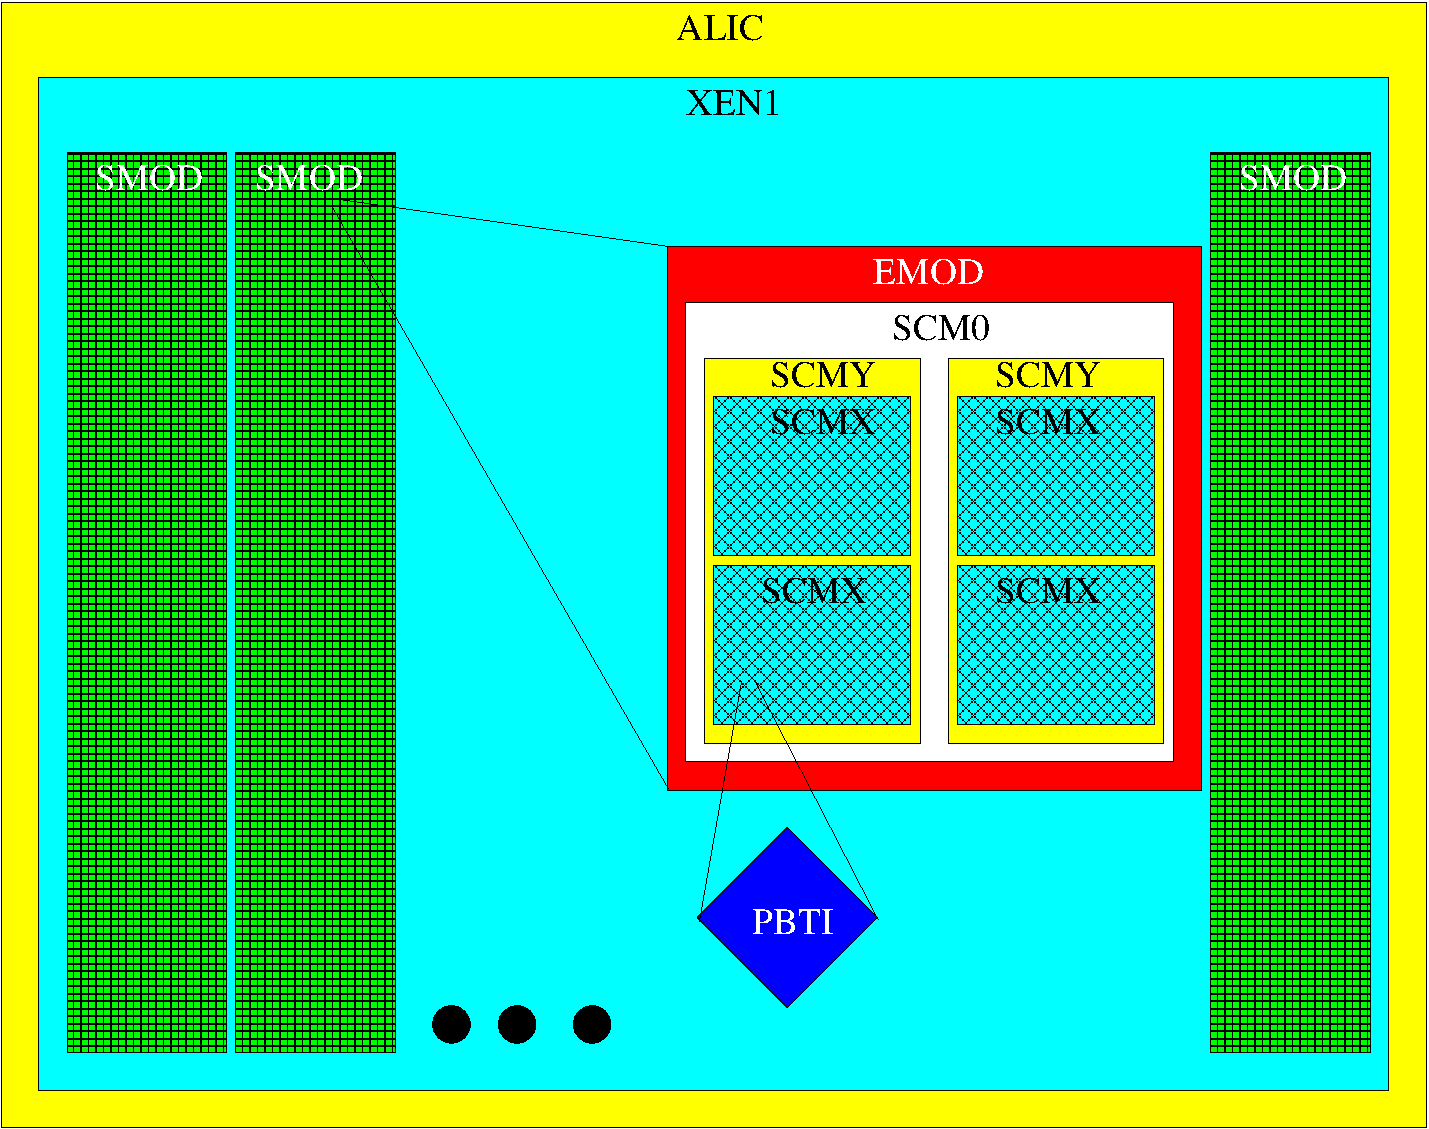
\includegraphics[width=0.8\textwidth]{figures/EMCalGeometryStructure.pdf}
\end{center}
\caption{\label{fig:GeometryDirectory}
Here is shown a typical hierarchical geometry structure. This
is similar to a directory structure except at each level one or
more copies, including translation and rotation operators, of
the daughters can be specified.}
\end{figure}

For the EMCal we do something a bit special (but not untypical
for a calorimeter using organic scintillators). We correct for 
the diminished light output
due to the ionization produced by the particles proceeding it.
This is done by rescaling the energy deposited using Birk's
law, equation \ref{equation:Birks}, as copied from GEANT3's 
\texttt{G3BRIRK} routine 
\cite{GEANT3:documentatoin}. This can be switched on or off
from the EMCal creation section of \texttt{Config.C} via
the \texttt{fBirkC0} variable in \texttt{AliEMCAL} class\footnote{
A function needs to be added to this class to allow for setting
this value and the Birk's law constants \texttt{fBirkC1}
and \texttt{fBirkC2}}.  There has been 
some debate about the proper way to deal with this in the
collaboration, mostly dealing with the limitations of any
Monte Carlo which transports particles one at a time, but
it has been agreed that including such a correction is
better than none at all.

\begin{eqnarray}
Light\; yield & = & 
 \frac{\Delta E_{deposited}}{1+C_1 \delta + C_2 \delta^2} 
\label{equation:Birks} \\
\delta & = & 
 \frac{1}{\rho}\frac{dE}{dx}\; \left[\frac{MeV\: cm^{2}}{g}\right]\nonumber \\
C_{1} & = & \left\{ \begin{array}{ll}
                    0.013\: \left[\frac{g}{MeV\;cm^{2}}\right] & Z=1 \\
                    0.00743\; \left[\frac{g}{MeV\; cm^{2}}\right] & 
                                         Z>1 \end{array}\right.\nonumber \\
C_{2} & = & 9.6\times 10^{-6}\; 
                  \left[\frac{g^{2}}{MeV^{2}\: cm^{4}}\right] \nonumber
\end{eqnarray}

The remaining tasks of the EMCal step manager is mostly book-keeping.
We only want to go to all of this effort if there is energy
being deposited in the sensitive scintillator volume, and not the
lead radiators or other structural materials. All of the relevant
information for the EMCal hit needs to be gathered. Lastly,
the \texttt{\bf AliEMCALHit} class needs to be created within the
\texttt{TClonesArray} of EMCal hits. This leads to some convoluted
looking code involving the TClonesArray fHits, the new
operator and the \texttt{AliEMCALHit} copy constructor (see
\texttt{\bf AliEMCAL::AddHit}).

The structure of these \texttt{EMCALHit} class (data structure) is
simple. It starts with the \texttt{AliHit} information which 
consists of the tTrack number of the track which entered 
the EMCal and its x,y,z global position (in cm). The EMCal specific
derivation includes the absolute tower ID where the hit signal is
from, the energy deposited by the showering particles
originating from this track in that tower, and the relative time
(with respect to the initial event) when this energy was deposited, 
the particle ID of the particle entering the EMCal, the entrance 
energy of the particle entering the EMCal, and the energy and 
momentum of the primary particle entering the EMCal.

Just a note, although not included in the code, the addition of
the signals from the APD, primarily due to neutrons interacting
with the APD, needs to be added. CMS has found that including
this effect measurably improves the response of their simulations.
This will require an addition to the EMCal step manager, but hopefully
not the \texttt{EMCALHit} structure.

\subsubsection{Step Manager and Monte Carlo Setting}
In the EMCal geometry description there are also settings done,
on a medium by medium basis, which are used in the non-EMCal
specific step manager code. In \texttt{AliEMCAL} where ever
a medium is defined (either by a call to \texttt{AliMedium}
or equivalently to a call to \texttt{TGeoMedium}) a list of
parameters must be given which effects the size of a step.
These parameters are given in Table \ref{tab:MediumParameers}.


\begin{longtable}{p{0.12\textwidth}p{0.1\textwidth}p{0.78\textwidth}}
  \multicolumn{3}{l}{Table \ref{tab:MediumParameers}} \\
      \hline \hline \\
      Type   & Variable  & Description \\ \hline
  \endfirsthead
      \multicolumn{3}{l}{\emph{Table \ref{tab:MediumParameers} continued}}\\
      \hline
      Type   & Variable & Description \\
      \hline
   \endhead
      \hline
       \multicolumn{3}{r}{\emph{Table \ref{tab:MediumParameers} continued 
                          on next page.}}
   \endfoot
      \hline \hline
      \caption{Parameters and flags defined in the EMCal geometry via
               a call to \texttt{ALIMedium} or \texttt{TGeoMedium}.
               Because we use a version of \texttt{GEANT3} 
               which has its geometrical modeler replaced by \texttt{TGeo}
               geometry, they are the same. This is also true for
               both \texttt{GEANT4}\cite{GEANT4} and 
               \texttt{Fluka}\cite{Fluka} particle
               transport Monte Carlos. See figure
               \ref{fig:emcalStepManager_ParticleStep} for
               a geometrical description of some of these parameters.
               This information comes from the 
               GEANT3 documentation CONS200-1 \cite{GEANT3:documentatoin}.
               \label{tab:MediumParameers}. 
       }
    \endlastfoot
    Int\_t & isvol & Sensitive volume flag.\newline
               0 Not a Sensitive volume.\newline
               1 Sensitive volume. \\
    Int\_t & ifield & Magnetic field flag. \newline
                     0 No magnetic field.\newline
                     -1 User decision in \texttt{guswim}. Not supported 
                        in AliRoot.\newline
                     1 Tracking performed with Runge Kutta.\newline
                     2 Tracking performed with helix. \newline
                     3 constant magnetic field along z.\\
    Float\_t & fieldm & Maximum magnetic field [kG].\\
    Float\_t & tmaxfd & Maximum deflection angle due to magnetic 
                       field [degrees].\\
    Float\_t & stemax & Maximum step allowed [cm].\\
    Float\_t & deemax & Maximum fractional energy loss in one step.\newline
                       $dee=\frac{\Delta E}{E_{k}}$\\
    Float\_t & epsil  & Tracking precision [cm].\newline
                       This effects transition to new volumes.\\
    Float\_t & stmin  & Minimum step due to continuous processes [cm].\newline
                       This must be set to 0 so that \texttt{GEANT3} will
                       computing it correctly. Not doing so will adversely
                       effect the simulation.\\
   \normalsize
   \label{tab:MediumParameers}
\end{longtable}


This isn't the whole story in regards to the step manager. There
are a number of things which we need to set/control that don't
appear in any EMCal code, but are dealt with in the transport
engines part of the step manager. Such settings and controls
are very dependent on the specific transport Monte Carlo being
used. All of these settings and controls have ALICE wide
default values, but most of them we will need to change to
get optimal performance and accuracy from our EMCal simulation. 
These switches and
settings are settable for specific materials. If a material
does not have a set of switches or settings set, the ALICE
wide defaults are used.

\begin{tabular*}{\textwidth}[ht]{p{.5\textwidth}p{0.5\textwidth}}
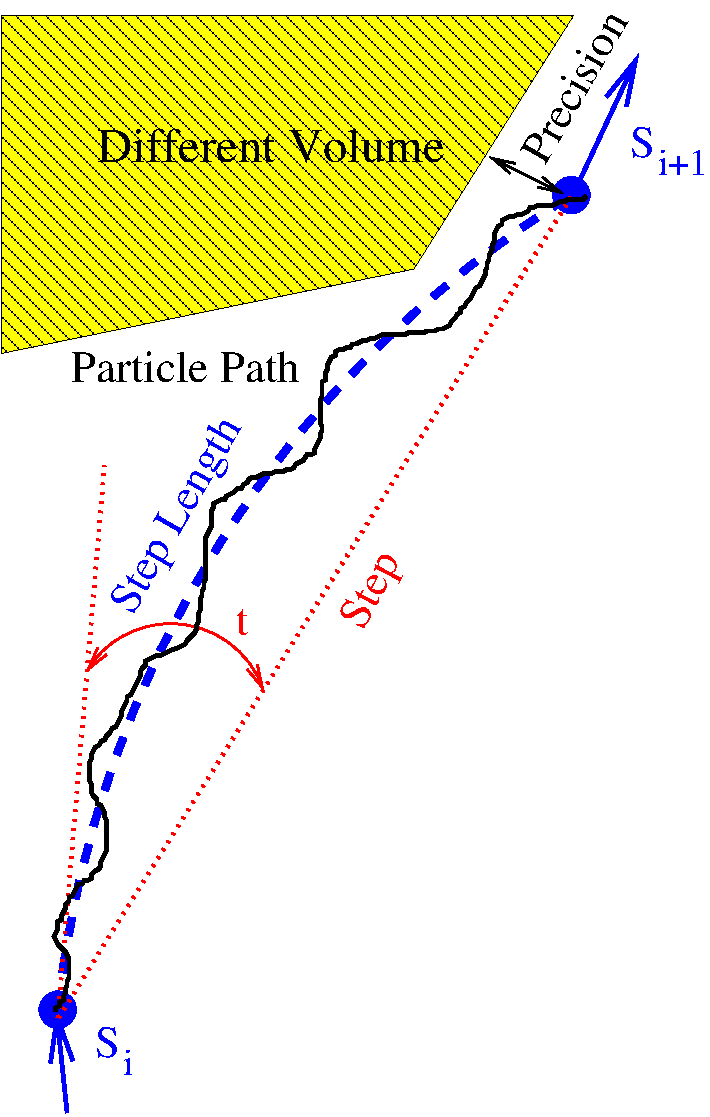
\includegraphics[width=0.5\textwidth]{figures/EMCalMCStep.pdf}
\label{fig:emcalStepManager_ParticleStep}
&
\vspace{-10.5cm}
Figure \ref{fig:emcalStepManager_ParticleStep}
An exaggerated Monte Carlo step showing some of the considerations associated
with transporting a Monte Carlo particle through a step. One step between
$s_{i}$ to $s_{i+1}$ is shown in the dotted (red) line. The dashed (blue)
line shows the step length taken due to a magnetic field. The solid (black)
line show what the particle path might really be. A new/different volume
is shown as the hashed (yellow) area. A new momentum and energy are
computed at the end of each step taking into account the energy loss
and multiple scattering. Also indicated is the deviation in the step
due to an applied magnetic field $t$, and the precision with which
the step has missed the other volume.
\\
\end{tabular*}


\paragraph{GEANT3 Switches and Settings}


GEANT3 was the first particle transport Monte Carlo integrated into
AliRoot and ROOT's virtual Monte Carlo and so has some of the
oldest and simplest interfaces. For simulation, AliRoot sets many
default settings and switches. This is done in \texttt{Config.C} which
you can find in \texttt{\$ALICE\_ROOT/macros}. There you will see a
number of line of the form \texttt{gMC->SetProcess(char *name,int value)}.
The switch names and there ALICE default values are shown in table
\ref{table:GEANT3PhysicsFlags}. There are limits both to the computer's
capabilities in dealing with the number of particles to transport and
with the physics models used by GEANT3. Consequently there are ``cuts''
used to stop the transport of particles which are below some energy
or are taking too long. The ALICE wide default values are also set
in \texttt{Config.C} using the function \texttt{gMC->SetCut(char *name,
double value)}. All of these values, and those included in the 
\texttt{galice.cuts} file are listed in table \ref{table:GEANT3PhysicsLimits}.

The \texttt{galice.cuts} file has a fixed format as indicated in
\texttt{\bf AliMC::ReadTransPar} function. In this file, lines
staring with an ``*'' are ignored. The remaining lines are required to
contain, in order separated by one or more spaces, Detector\_Name, 
Detector's\_media\_number, and then the numbered cuts and flags listed in
tables \ref{table:GEANT3PhysicsFlags} and \ref{table:GEANT3PhysicsLimits}.

\begin{longtable}{p{0.12\textwidth}p{0.1\textwidth}p{0.78\textwidth}}
  \multicolumn{3}{l}{Table \ref{table:GEANT3Switchs}} \\
      \hline \hline \\
      Switch   & \small ALICE Default values & Description \\ \hline
  \endfirsthead
      \multicolumn{3}{l}{\emph{Table \ref{table:GEANT3Switchs} continued}}\\
      \hline
      Switch   & \small ALICE Default value & Description \\
      \hline
   \endhead
      \hline
       \multicolumn{3}{r}{\emph{Table \ref{table:GEANT3Switchs} continued 
                          on next page.}}
   \endfoot
      \hline \hline
      \caption{
      %\multicolumn{3}{p{0.95\textwidth}}{Table \ref{table:GEANT3Switches}: 
               \label{table:GEANT3Switchs}GEANT3 physics process flags. 
                These flags can be set on a 
                material by material basis. The ALICE Default values are 
                set in the \texttt{Config.C} file uses the 
                \texttt{gMC->SetProcess} 
                function. The setting of these specific flags for any 
                specific material is done in 
                \texttt{\$ALICE\_ROOT/data/galice.cuts}
                file. The number on the left of the switch name is the
                column in the \texttt{galice.cuts} file that this switch
                is expected to be found. This information comes from the 
                GEANT3 documentation PHYS001-3 \cite{GEANT3:documentatoin}. 
       }
    \endlastfoot
    \footnotesize
    13 ANNI & 1 & Positron annihilation. The $e^+$ is stopped.\newline
               0 No position annihilation.\newline
               1 Positron annihilation with generation of $\gamma$.\newline
               2 Positron annihilation without generation of $\gamma$.\\
    \footnotesize
    14 BREM & 1 & bremsstrahlung. The interaction particle ($e^-$, $e^+$, 
                $\mu^-$, $\mu^+$) is stopped.\newline
               0 No bremsstrahlung. \newline
               1 bremsstrahlung with generation of $\gamma$.\newline
               2 bremsstrahlung without generation of $\gamma$.\\
    \footnotesize
    15 COMP & 1 & Compton scattering.\newline
               0 No Compton scattering.\newline
               1 Compton scattering with generation of $e^-$. \newline
               2 Compton scattering without generation of $e^-$.\\
    \footnotesize
    16 DCAY & 1 & Decay in flight. The decaying particles stops. \newline
               0 No decay in flight \newline 
               1 Decay in flight with generation of secondaries \newline
               2 Decay in flight without generation of secondaries \\
    \footnotesize
    17 DRAY & 0 & $\delta$-ray production.\newline
               0 No $\delta$-ray production.\newline
               1 $\delta$-ray production with generation of $e^-$.\newline
               2 $\delta$-ray production without generation of $e^-$.\\
    \footnotesize
    18 HADR & 1 & Hadronic interactions. The particle is stopped in case 
                of inelastic interactions, while it is not stopped in case 
                of elastic interactions.\newline
               0 No hadronic interactions.\newline
               1 Hadronic interactions with generation of secondaries.\newline
               2 Hadronic interactions without generation of 
                 secondaries.\newline
               $>2$ can be used in the user code \texttt{GUPHAD} and 
                 \texttt{GUHADR} to choose 
                 a hadronic package. These values have no effect on the 
                 hadronic packages themselves. Not supported in AliRoot.\\
    \footnotesize
    19 LOSS & 2 & Continuous energy loss.\newline
               0 No continuous energy loss, DRAY is forced to 0.\newline
               1 Continuous energy loss with generation of $\delta$-rays 
                  which have an energy above DCUTE and restricted 
                  Landau-fluctuations\cite{LandauFluct} for $\delta$-rays 
                  which have an 
                  energy below DCUTE (no $\delta$-ray produced).\newline
               2 Continuous energy loss without generation of $\delta$-rays 
                  and full Landau-Vavilov-Gauss\cite{LandauVavilov} 
                  fluctuations. In this case 
                  DRAY is forced to 0 to avoid double counting of 
                  fluctuations.\newline
               3 Same as 1, kept for backwards compatibility.\newline
               4 Energy loss without fluctuations. The value obtained 
                 from the tables is used directly.\\
    \footnotesize
    20 MULS & 1 & Multiple scattering.\newline
               0 No multiple scattering.\newline
               1 Multiple scattering according to Moliere\cite{Moiere} 
                 theory.\newline
               2 Same as 1. Kept for backwards compatibility.\newline
               3 Pure Gaussian scattering according to the Rossi 
                 formula\cite{Rossi}.\\
    \footnotesize
    21 PAIR & 1 & Pair production. The interacting $\gamma$ is 
                  stopped. \newline
               0 No pair production. \newline
               1 Pair production with generation of $e^+/e^-$.\newline
               2 Pair production without generation of $e^+/e^-$.\\
    \footnotesize
    22 PHOT & 1 & Photoelectric effect. The interacting photon is 
                  stopped.\newline
               0 No photo-electric effect. \newline
               1 Photo-electric effect with generation of $e^-$.\newline
               2 Photo-electric effect without generation of $e^-$.\\
    \footnotesize
    23 RAYL & 1 & Rayliegh effect\cite{Rayligh}. The interacting 
                  $\gamma$ is not stopped.\newline
               0 No Raylieght effect.\newline
               1 Rayliegh effect.\\
    \footnotesize
    24 STRA & 0 & Turns on the collision sampling method to simulate 
                  energy loss in thin materials, particularly gasses.\newline
               0 Collision sampling is off.\newline
               1 Collision sampling is on. \\
    \footnotesize
    PFIS & 0 & Nuclear fission induced by a photon The photon stops.\newline
               0 No photo-fission.\newline
               1 Photo-fission with generation of secondaries.\newline
               2 Photo-fission without generation of secondaries.\\
    \footnotesize
    MUNU & 1 & Muon-nucleus interactions. The muon is not stopped.\newline
               0 No muon-nucleus interactions.\newline
               1 Muon-nucleus interactions with generation of 
                 secondaries.\newline
               2 Muon-nucleus interactions without generation of secondaries.\\
    \footnotesize
    CKOV & 1 & Light absorption. This process is the absorption of light 
                photons in dielectric materials. It is turned on by default 
                when the generation of $\check{C}$erenkov\cite{Cerenkov} 
                light is requested (in GEANT manual it is LABS).\newline
                0 No absorption of photons.\newline
                1 Absorption of photons with possible detection.\\
    \footnotesize
    SYNC & 0 & Synchrotron radiation in magnetic fields.\newline
               0 Synchrotron radiation is not simulated.\newline
               1 Synchrotron photon are generated, at the end of the 
                 tracking step.\newline
               2 Photons are not generated, the energy is deposited 
                 locally.\newline
               3 Synchrotron photons are generated, distributed along the 
                 curved path of their particle. \\
   \normalsize
   \label{table:GEANT3PhysicsFlags}
\end{longtable}

\begin{longtable}{p{0.15\textwidth}p{0.2\textwidth}p{0.65\textwidth}}
  \multicolumn{3}{l}{Table \ref{table:GEANT3PhysicsLimits}} \\
      \hline \hline \\
      Parameter   & \small ALICE Default value & Description \\ \hline
  \endfirsthead
      \multicolumn{3}{l}{\emph{Table \ref{table:GEANT3PhysicsLimits} 
                         continued}}\\
      \hline
      Parameter   & ALICE Default value & Description \\
      \hline
   \endhead
      \hline
       \multicolumn{3}{r}{\emph{Table \ref{table:GEANT3PhysicsLimits} 
                          continued on next page.}}
   \endfoot
      \hline \hline
      \caption{\label{table:GEANT3PhysicsLimits}GEANT3 physics process limits. 
                These ``cuts'' can be set on a 
                material by material basis. The ALICE Default values are 
                set in the \texttt{Config.C} file uses the 
                \texttt{gMC->SetCuts} 
                function. The setting of these specific flags for any 
                specific material is done in 
                \texttt{\$ALICE\_ROOT/data/galice.cuts}
                file. The number on the left of the cut name is the
                column in the \texttt{galice.cuts} file that this cut
                is expected to be found. This information comes from the 
                GEANT3 documentation ZZZZ010-2 \cite{GEANT3:documentatoin}
      }
    \endlastfoot

    \footnotesize
    3 CUTGAM & $1.\times 10^{-3}$ GeV & Threshold for gamma transport.\\
    \footnotesize
    4 CUTELE & $1.\times 10^{-3}$ GeV & Threshold for electron and positron 
                                   transport.\\
    \footnotesize
    5 CUTNEU & $1.\times 10^{-3}$ GeV & Threshold for neutral hadron 
                                         transport.\\
    \footnotesize
    6 CUTHAD & $1.\times 10^{-3}$ GeV & Threshold for charged hadron 
                                        and ion transport.\\
    \footnotesize
    7 CUTMUO & $1.\times 10^{-3}$ GeV & Threshold for muon transport.\\
    \footnotesize
    8 BCUTE &  $1.\times 10^{-3}$ GeV & Threshold for photons produced by 
                                   electron bremsstrahlung.\\ 
    \footnotesize
    9 BCUTM &  $1.\times 10^{-3}$ GeV & Threshold for photons produced by 
                                   muon bremsstrahlung.\\ 
    \footnotesize
    10 DCUTE &  $1.\times 10^{-3}$ GeV & Threshold for electrons produced by 
                                    electron $\delta$-rays.\\ 
    \footnotesize
    11 DCUTM &  $1.\times 10^{-3}$ GeV & Threshold for electrons produced by 
                                    muon or hadron $\delta$-rays.\\ 
    \footnotesize
    12 PPCUTM & $1.\times 10^{-3}$ GeV & Threshold for $e^{\pm}$ direct pair 
                                    production by muons.\\
    \footnotesize
    TOFMAX & $1.\times 10^{10}$ sec & Threshold on time of flight counted 
                                       from primary interactions time.\\ 

   \label{table:GEANT3PhysicsLimits}
\end{longtable}

\paragraph{GEANT4 Switches and Settings}

\paragraph{Fluka Switches and Settings}

%
\begin{thebibliography}{99}
\bibitem{GEANT3:documentatoin} CERN Program Library. 
         \textsl{GEANT Detector description and Simulation Tool},
         CERN Program Library Long writeup W5013, October 1994
\bibitem{GEANT4} GEANT4 Working Group, ``User Documentation'',
                 Accessed Feb. 4 2013. 
                 http://geant4.cern.ch/support/suerdocumentatoin.shtml
\bibitem{Fluka}  FLUKA Team, ``FLUKA'', Access Feb. 4 2013,
                 http://www.fluka.org/fluka.php?id=man\_onl
\bibitem{LandauFluct} \textsl{GEANT Detector description and Simulation Tool},
                      PHYS332. and
                      L. Landau. \textsl{On the Energy Loss of Fast Particles 
                      by Ionisation}, J. Phys. 8:201, 1944. and
                      K. S. K$\ddot{o}$lbig and B. Schorr. \textsl{Asymptotic 
                      expansion for the Landau density and distribution 
                      functions}, Comp. Phys. Comm., 32:121,1984
\bibitem{LadauVavilov}\textsl{GEANT Detector description and Simulation Tool},
                       PHYS332. and 
                       P. V. Valilov. \textsl{Ionisation losses of high 
                       energy heavy particles}, Soviet Physics 
                       JETP, 5:749, 1957
\bibitem{Moliere}\textsl{GEANT Detector description and Simulation Tool},
                 PHYS320. and
                 G. Z. Moliere \textsl{Theorie de Streuung schneller 
                 geladener Teilchen I: Enzelstreuung am abgerschmitten 
                 Coulomb-Feld},Z. Naturforsch., 2a:133, 1947 and
                 G. Z. Moliere, \textsl{Teeorie der Steuung schneller 
                 geladerner Teichen II: Merfach- und Vielfachstreuung} 
                 Z. Naturforsh., 3a:87, 1948 and
                 W. T. Scott. Rev. Mod. Phys. 35:231 1963
\bibitem{Rossi}\textsl{GEANT Detector description and Simulation Tool},
                 PHYS320 and
                 R. Rossi, Prentice-Hall, Englewoood Clifgs, 1962
                 R. Rossi, and K. Greisen, Rev. Mod. Physics, 13-240, 1942
\bibitem{Rayliegh} \textsl{GEANT Detector description and Simulation Tool},
                   PHYS250. and
                   W. R. Nelson, H. Hiayama, and D. W. O. Rogers. Technical 
                   Report 265, SLAC, 1985
\bibitem{Cerenkov} \textsl{GEANT Detector description and Simulation Tool},
                   PHYS260,
                   J. D. Jackson \textsl{Classical Electrodyanamics}, 
                   J. Wiley et Sons, Inc. New York, 1975
\end{thebibliography}
%
%\end{document}
%

\clearpage


\subsection{Digitization: SDigits and Digits - Evi \label{sec:digi}}

We want to generate events which look like the real data collected
by the experiment. In the end, we want to have an amplitude in ADC
counts and a time (when particle traverse a cell) per each cell (tower)
of the calorimeter. In the code for calorimeters, it is done in the
following steps: 
\begin{enumerate}
\item \textbf{SDigit} objects are created, they consist
of the sum of deposited energy by all Hits in a cell (a particle can
create Hits in different cells but only one in a single cell), so
there is only one SDigit per fired cell.
\item \textbf{Digit} objects are created, they are like the SDigits but the energy in the cell
is transformed into the ADC amplitude units, the electronic noise
is added and Digits whose energy does not pass an energy threshold
(3 ADC counts) are eliminated. SDigits and Digits are stored in the files
\textbf{EMCAL.SDigits.root} and \textbf{EMCAL.Digits.root}, respectively.
\end{enumerate}

\subsection{Raw data - David \label{sec:simu_raw}}

The experiment does not record Digits directly, but instead a series of so-called
time samples with 10-bit ADC counts per channel. Each time bin is 100 ns
wide, corresponding to a 10 MHz readout.
These samples are referred to as
\textbf{Raw Data}. The samples follow a certain signal shape, more complicated than
a Gaussian distribution, which is fitted offline. 
The simulated signal (Gamma-2) shape is described in the AliEMCALRawResponse class,
in the RawResponseFunction method.
With real data, which is zero-suppressed, i.e. has the pedestal subtracted online, the
Digits amplitude is just the maximum of the distribution obtained
with the fit to the sample. The Digit time (defined by the time the
particle hits the active volume of the detector) is the time value at
the maximum signal fit. There are methods to go from Digits to
Raw and vice versa in the AliEMCALRawUtils class: Raw2Digits and Digits2Raw,
respectively. For the reconstruction step Digits are needed. The
generation of Raw Data is optional during simulations and the generated 
data can be reconstructed directly from Digits, but Raw data is the initial
step when reconstructing real data.


\subsection{How to make a simulation\label{sec:simu_steps}}

TestEMCALSimulation.C is a very simple macro where we specify all the simulation parameters
and proccess the simulation. Below is a similar but a bit more elaborated macro:



\begin{DDbox}{\linewidth}
\begin{lstlisting}
void TestEMCALSimulation() {

TString detector=``EMCAL TPC''; // Define in this variable the detectors that you want to be included in the simulation for the digitization. They can be less detectors than the detectors defined in the Config.C file, imagine that you want all the detectors in front of EMCal present to consider the conversion of particles but you are not really interested in the output from these detectors. 
// Option detector=``ALL''  makes all detectors. 

AliSimulation sim ; //Create simulation object 

// Generation and simulation 

sim.SetRunGeneration(kTRUE) ; //Default value is kTRUE, make generation  
// For some reason we may want to redo the Digitization, without redoing the generation, in this case it must set to kFALSE 

// Making SDigits 
sim.SetMakeSDigits(detector) ; //We want to make SDigits
// set no detectors if SDigits are already made

// Making Digits 
sim.SetMakeDigits(detector) ; //We want to make Digits 
// set no detectors if SDigits are already made

//Merging 
//sim.MergeWith(``bgrd/galice.root'') ; //If we want to merge a signal and a background, the merging is done at the SDigit level. The background must be located in the repertory defined in the method. 

//Write Raw Data, make Raw data from digits 
//sim.SetWriteRawData(detector) ;
//sim.SetConfigFile(``somewhere/ConfigXXX.C'');//Default is Config.C

//Make the simulation 
sim.Run(3) ; // Run the simulation and make 3 events 



\end{lstlisting}
\end{DDbox}